\documentclass[a4paper]{article}
\usepackage[margin=2cm]{geometry}

\usepackage{polski}
\usepackage[utf8]{inputenc}
\usepackage[polish]{babel}

\usepackage{color, colortbl}
\usepackage[dvipsnames]{xcolor}
\usepackage{listings}
\usepackage{graphicx}

\usepackage{setspace}

\usepackage{natbib}

\lstset{literate=%
{ą}{{\k{a}}}1
{ć}{{\'c}}1
{ę}{{\k{e}}}1
{ł}{{\l{}}}1
{ń}{{\'n}}1
{ó}{{\'o}}1
{ś}{{\'s}}1
{ż}{{\.z}}1
{ź}{{\'z}}1
{Ą}{{\k{A}}}1
{Ć}{{\'C}}1
{Ę}{{\k{E}}}1
{Ł}{{\L{}}}1
{Ń}{{\'N}}1
{Ó}{{\'O}}1
{Ś}{{\'S}}1
{Ż}{{\.Z}}1
{Ź}{{\'Z}}1,
language=c++,
keywordstyle=\color{gray},
commentstyle=\color{lightgray},
stringstyle=\color{lightgray},
numbers=left,
frame=TBlr,
breaklines=true,
tabsize=2,
numberstyle=\tiny,
basicstyle=\footnotesize \ttfamily
}

\renewcommand\thesection{\arabic{section}.}
\renewcommand\thesubsection{\thesection\arabic{subsection}.}
\renewcommand\thesubsubsection{\thesubsection\arabic{subsubsection}.}
\renewcommand\theparagraph{\thesubsubsection\arabic{paragraph}.}
\renewcommand\thesubparagraph{\theparagraph\arabic{subparagraph}.}

\title{Projekt  - inżynieria E-systemów w technologii JAVA \\ Aplikacja zarządzająca wydarzeniami kulturalnymi.}
\author{\textbf{Przemysław Michalak} 181101\\ 
\textbf{Krystian Horecki} 181079 \\
\textbf{Grupa C} (śr. 11.15) \\ \\ Politechnika Wrocławska}
\date{19.03.2012 r.}


\begin{document}

\maketitle
\tableofcontents

\newpage

\section{Schemat bazy danych}
Poniżej na rysunku \ref{baza} zamieszczony został schemat bazy danych, zawierającej wszystkie wymagane do działania aplikacji
elementy.
Każde pole w bazie zostało na nim wstępnie opisane.
Na podstawie poniższego schematu w dużej mierze oparta zostanie późniejsza aplikacja.

\begin{figure}[!h]
\begin{center}
  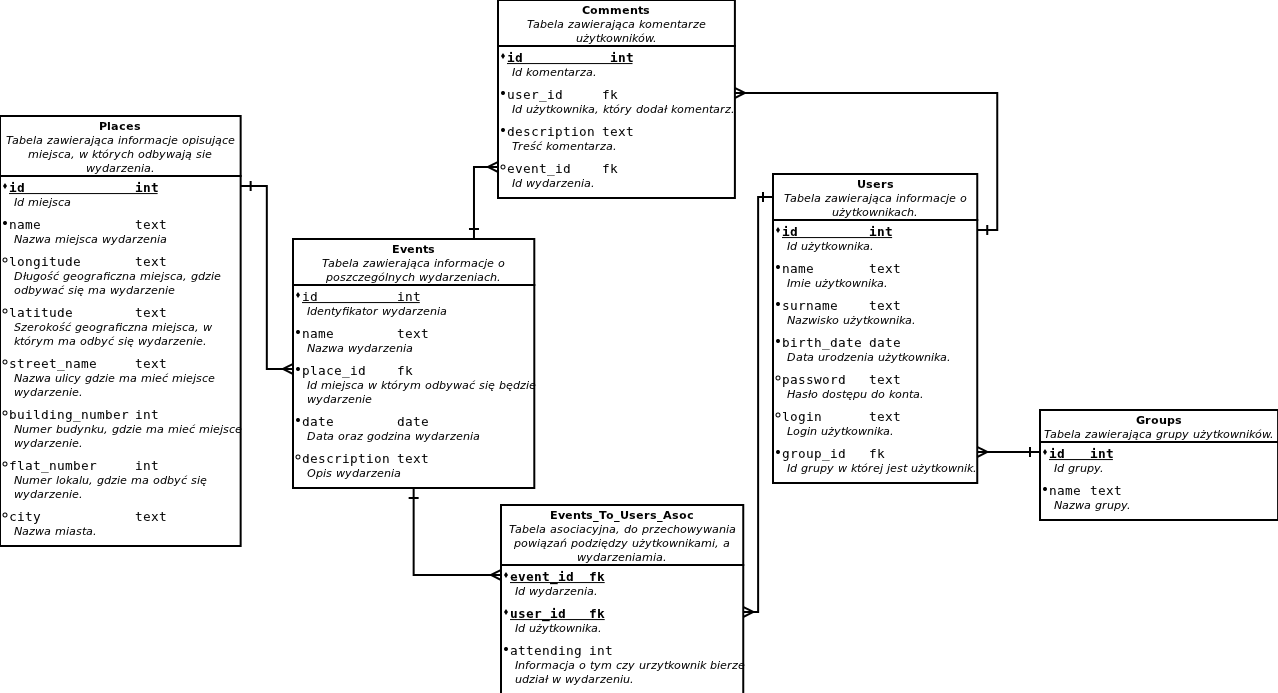
\includegraphics[width=\textwidth]{baza.png}
  \caption{Schemat bazy danych dla aplikacji}
  \label{baza}
\end{center}
\end{figure}

\pagebreak
\section{Diagram klas aplikacji}
Poniższy diagram przedstawiony na rysunku \ref{klasy} pokazuje uproszczoną, abstrakcyjną strukturę aplikacji.
Przedstawione na nim zależności pokazują strukturę w jakiej zorganizowany został przepływ danych w naszej aplikacji.
Pozwala on na oddzielenie funkcjonalności związanej z bezpośrednią obsługą prostych zapytań do bazy danych, od bardziej skomplikowanych
operacji biznesowych.


\begin{figure}[!h]
\begin{center}
  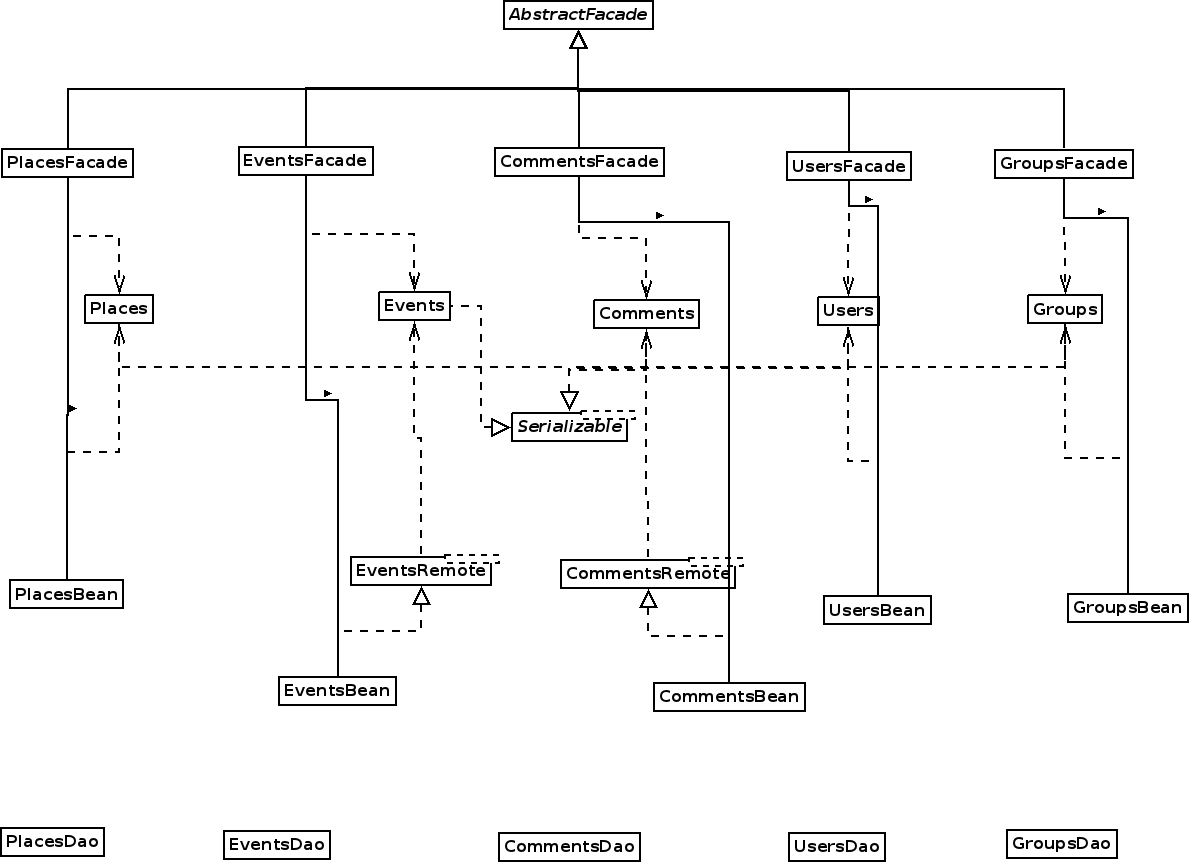
\includegraphics[width=\textwidth]{classDiagram.png}
  \caption{Diagram klas dla aplikacji}
  \label{klasy}
\end{center}
\end{figure}

\pagebreak
\section{Lista testów dla aplikacji}
Testy, które przewidziane zostały dla naszej aplikacji w głównej mierze opierając się na grupowaniu na 
części zależne od typu danych na jakich operujemy.
W naszym wypadku w głównej mierze chcielibyśmy testować funkcjonalności związane z operacjami dodawania oraz pobierania informacji 
na temat wydarzeń.

Testy związane z wydarzeniami:
\begin{itemize}
 \item Dodawanie kilku wydarzeń dla konkretnej daty, a następnie pobieranie ich.
 \item Pobieranie wcześniej dodanych wydarzeń dla konkretnego miasta.
 \item Dodawanie osób do wydarzenia, a następnie sprawdzanie poprawności dodania.
 \item Sprawdzanie poprawności parsowania zadanego pliku w formacie html, będącego bazą dla wydarzeń.
 \item Sprawdzanie poprawności zwracanych wydarzeń przeszłych oraz przyszłych
 \item Sprawdzanie usuwania użytkowników z wydarzenia.
\end{itemize}


Oprócz oczywistych przypadków sprawdzania poprawności operacji przewidziane są także
przypadki sprawdzania działania aplikacji, gdy wczytane zostaną niepoprawne dane lub wykonana zła operacja.
\begin{itemize}
 \item Sprawdzanie poprawności formatu współrzędnych
 \item Sprawdzanie poprawności daty wydarzenia
\end{itemize}

 


\end{document} 




